%**************************************************************************************
% License:
% CC BY-NC-SA 4.0 (http://creativecommons.org/licenses/by-nc-sa/4.0/)
%**************************************************************************************

\documentclass[notes]{beamer}

\mode<presentation> {

\usetheme{Madrid}

% Burnt orange
\definecolor{burntorange}{rgb}{0.8, 0.33, 0.0}
\colorlet{beamer@blendedblue}{burntorange}
% Pale yellow
\definecolor{paleyellow}{rgb}{1.0, 1.0, 0.953}
\setbeamercolor{background canvas}{bg=paleyellow}
% Secondary and tertiary palette
\setbeamercolor*{palette secondary}{use=structure,fg=white,bg=burntorange!80!black}
\setbeamercolor*{palette tertiary}{use=structure,fg=white,bg=burntorange!60!black}

% To remove the navigation symbols from the bottom of all slides uncomment this line
%\setbeamertemplate{navigation symbols}{}
}

% Custom note page template for longer notes
\setbeamertemplate{note page}{%
  \insertnote
}
\setbeameroption{show notes}

\usepackage{amsmath}
\DeclareMathOperator*{\argmin}{arg\,min}
\DeclareMathOperator*{\argmax}{arg\,max}
\usepackage{bm}
\usepackage{booktabs}
\usepackage{breqn}
\usepackage{cleveref}
\usepackage{graphicx}
\usepackage[labelsep=space,tableposition=top]{caption}
\renewcommand{\figurename}{Fig.}
\usepackage{caption,subcaption}
\usepackage{xcolor}
\usepackage{hyperref}
\usepackage{tikz}
\usetikzlibrary{positioning,calc}

%\AtBeginSection[]{
%	\begin{frame}{Outline}
%		\tableofcontents[
%		currentsection,
%		hideallsubsections
%		]
%	\end{frame}
%}

%----------------------------------------------------------------------------------------
%	TITLE PAGE
%----------------------------------------------------------------------------------------
\title[Neural ODEs]{Neural Ordinary Differential Equations}
\author{Krishna Kumar}
\institute[UT Austin]
{
University of Texas at Austin \\
\medskip
\textit{
  \url{krishnak@utexas.edu}}
}
\date{}

\begin{document}

\begin{frame}
\titlepage
\end{frame}

\begin{frame}
 \frametitle{Overview}
 \tableofcontents
\end{frame}

%----------------------------------------------------------------------------------------
% SLIDES
%----------------------------------------------------------------------------------------

\section{From ResNets to Continuous Dynamics}

%------------------------------------------------
\begin{frame}
\frametitle{Learning Objectives}

\begin{itemize}
    \item Understand the connection between ResNets and continuous dynamics
    \item Master the Neural ODE framework and adjoint method
    \item Implement ODENets for image classification
    \item Apply continuous normalizing flows for generative modeling
    \item Build latent ODE models for irregular time series
\end{itemize}

\vspace{1cm}
\centering
\href{https://colab.research.google.com/github/kks32-courses/sciml/blob/main/docs/07-neural-ode/neural-ode.ipynb}{\beamergotobutton{Open Notebook}}

\end{frame}

%------------------------------------------------
\begin{frame}
\frametitle{The ResNet Formula}

A residual network transforms hidden states layer by layer:

\begin{equation}
h_{t+1} = h_t + f(h_t, \theta_t)
\end{equation}

where $t \in \{0, 1, \ldots, T\}$ indexes the layers.

\vspace{0.5cm}

\begin{block}{The Key Question}
What happens as we add more layers ($T \to \infty$) and take smaller steps?
\end{block}

\note{
Let's understand why this question matters. In a ResNet, we're adding a small correction $f(h_t, \theta_t)$ to our hidden state. Think of this like taking steps on a path: we're at position $h_t$, and we move by some amount $f(h_t, \theta_t)$.

Now imagine we make our layers shallower -- each one does less work. To compensate, we add more layers. In the limit, each layer does an infinitesimally small update, but we have infinitely many of them.

This is exactly the setup for calculus! When we have many small discrete steps, we get a continuous process. The transformation becomes: $h_{t+1} - h_t = f(h_t, \theta_t)$. If we divide by the step size $\Delta t = 1$ and take the limit as steps become infinitesimal, we get $\frac{dh}{dt} = f(h, \theta)$.

This connection means: ResNets with many layers $\approx$ following a continuous path through hidden state space.
}

\end{frame}

%------------------------------------------------
\begin{frame}
\frametitle{The Euler Connection}

The ResNet update is the \textbf{Euler discretization} of an ODE:

\begin{equation}
\frac{dh(t)}{dt} = f(h(t), t, \theta)
\end{equation}

\vspace{0.5cm}

\begin{alertblock}{Key Insight}
A ResNet with infinitely many infinitesimal layers $\equiv$ solving an ODE
\end{alertblock}

\vspace{0.5cm}

Instead of specifying discrete layers, we parameterize the \textbf{derivative} of the hidden state using a neural network.

\note{
Here's the beautiful shift in perspective. In traditional neural networks, we explicitly define what happens at each layer. In Neural ODEs, we instead define \emph{how the hidden state changes}.

Think of it like describing motion: instead of saying ``at time 1 you're at position $x_1$, at time 2 you're at position $x_2$,'' we say ``your velocity is $v(x, t)$'' and let calculus figure out where you'll be.

The function $f(h(t), t, \theta)$ is our neural network. It takes the current hidden state and time, and outputs the instantaneous rate of change. To get the hidden state at any time $t_1$, we solve:
$$h(t_1) = h(t_0) + \int_{t_0}^{t_1} f(h(t), t, \theta) \, dt$$

This is fundamentally different from ResNets: the network depth becomes a continuous quantity. We're not limited to discrete layers anymore. The ODE solver adaptively determines how many ``function evaluations'' are needed for a given accuracy tolerance.
}

\end{frame}


%------------------------------------------------
\begin{frame}
	\frametitle{ResNet vs ODE}
	
	\begin{center}
		\includegraphics[width=0.7\textwidth]{figs/neuralode.png}
	\end{center}

\end{frame}

%------------------------------------------------
\begin{frame}
	\frametitle{ResNet vs ODE}

	\begin{center}
		\includegraphics[width=0.7\textwidth]{figs/resent-neuralode-arch.png}
	\end{center}

\end{frame}

%------------------------------------------------
\begin{frame}
\frametitle{Numerical Integration: From Discrete to Continuous}

\textbf{The Mathematician's View:}

The exact solution to $\frac{dx}{dt} = f(x, t, \theta)$ from time $t_k$ to $t_{k+1}$ is:

\begin{equation}
x_{k+1} = x_k + \int_{t=t_k}^{t=t_{k+1}} f(x(\tau), \tau, \theta) \, d\tau
\end{equation}

\vspace{0.3cm}

\textbf{The Problem:} We can't compute this integral analytically!

\vspace{0.3cm}

\textbf{The Solution:} Numerical integration schemes approximate this integral

\begin{itemize}
    \item \textbf{Euler (ResNet):} Simplest approximation, worst accuracy
    \item \textbf{Runge-Kutta:} Better approximations, higher accuracy
    \item \textbf{Adaptive methods:} Adjust step size automatically
\end{itemize}

\note{
\textbf{Understanding the Integral:} When we write $x_{k+1} = x_k + \int_{t_k}^{t_{k+1}} f(x(\tau), \tau, \theta) d\tau$, we're saying: "To get from $x_k$ to $x_{k+1}$, we need to accumulate all the infinitesimal changes $f(x(\tau), \tau) d\tau$ along the entire trajectory from time $t_k$ to $t_{k+1}$."

The variable $\tau$ is a dummy integration variable that runs from $t_k$ to $t_{k+1}$. At each instant $\tau$, we evaluate the vector field $f$ at the current state $x(\tau)$.

\textbf{Why Numerical Integration?} For most neural networks $f$, this integral has no closed-form solution. We must approximate it numerically.

\textbf{The Key Tradeoff:} More accurate integrators require more function evaluations of $f$, which means more forward passes through the neural network. But they give better approximations of the true solution.

\textbf{Neural ODE's Advantage:} Because we're approximating the continuous integral, we can choose different integration schemes based on our needs:
\begin{itemize}
\item Fast but rough? Use Euler
\item Accurate? Use RK4 or Dormand-Prince
\item Need energy conservation? Use symplectic integrators
\end{itemize}

ResNets are stuck with Euler (one step, $\Delta t = 1$), but Neural ODEs can use any integrator!
}

\end{frame}

%------------------------------------------------
\begin{frame}
\frametitle{Integration Schemes: Euler (ResNet)}

\textbf{Euler Method (Forward Euler):}
\begin{equation}
x_{k+1} = x_k + \Delta t \cdot f(x_k, t_k, \theta)
\end{equation}

With $\Delta t = 1$: $x_{k+1} = x_k + f(x_k, \theta)$ \quad $\leftarrow$ ResNet!

\vspace{0.5cm}

\begin{center}
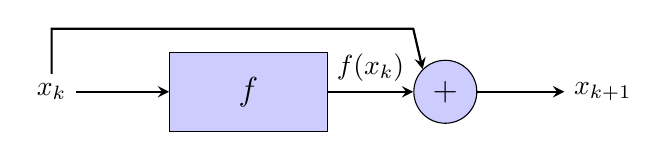
\begin{tikzpicture}[
    block/.style={rectangle, draw, fill=blue!20, minimum width=2cm, minimum height=1cm, font=\large},
    sum/.style={circle, draw, fill=blue!20, minimum size=0.8cm, font=\large},
    arrow/.style={->, >=stealth, thick}
]
    \node (input) at (0,0) {$x_k$};
    \node[block] (f) at (2.5,0) {$f$};
    \node[sum] (add) at (5,0) {$+$};
    \node (output) at (7,0) {$x_{k+1}$};

    \draw[arrow] (input) -- (f);
    \draw[arrow] (f) -- (add) node[midway, above] {$f(x_k)$};
    \draw[arrow] (add) -- (output);
    \draw[arrow] (input) |- ($(add.west) + (0,0.8)$) -- (add.north west);
\end{tikzpicture}
\end{center}

\vspace{0.3cm}

\textbf{Properties:}
\begin{itemize}
    \item One function evaluation per step
    \item First-order accurate: error $\mathcal{O}(\Delta t^2)$
    \item Simple but can be unstable
\end{itemize}

\note{
\textbf{Euler Method Explained:} The simplest approximation of $\int_{t_k}^{t_{k+1}} f(x(\tau)) d\tau$ is to assume $f$ is constant over the interval:
$$\int_{t_k}^{t_{k+1}} f(x(\tau)) d\tau \approx f(x_k) \cdot (t_{k+1} - t_k) = f(x_k) \cdot \Delta t$$

This is like approximating the area under a curve with a single rectangle (left Riemann sum).

\textbf{The Block Diagram:}
\begin{itemize}
\item Input $x_k$ goes into function $f$ (the neural network)
\item Output $f(x_k)$ is the instantaneous rate of change
\item Add this change to the current state $x_k$
\item Result is $x_{k+1} = x_k + f(x_k)$
\end{itemize}

\textbf{Why ResNets Use This:} ResNets weren't designed for differential equations. The residual connection $x_{k+1} = x_k + f(x_k)$ just happens to be Euler's method with $\Delta t = 1$.

\textbf{The Problem with Euler:}
\begin{itemize}
\item Large error accumulation over many steps
\item Can become unstable for stiff equations
\item First-order accuracy means doubling steps only halves the error
\end{itemize}

For Neural ODEs, we can do much better!
}

\end{frame}

%------------------------------------------------
\begin{frame}
\frametitle{Integration Schemes: Midpoint (2nd Order)}

\textbf{Midpoint Method (2nd order Runge-Kutta):}
\begin{align}
k_1 &= f(x_k, t_k, \theta) \\
x_{k+1} &= x_k + \Delta t \cdot f(x_k + \tfrac{\Delta t}{2} k_1, t_k + \tfrac{\Delta t}{2}, \theta)
\end{align}

\vspace{0.3cm}

\begin{center}
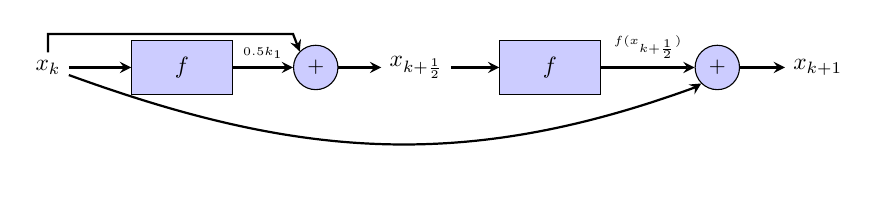
\begin{tikzpicture}[
    block/.style={rectangle, draw, fill=blue!20, minimum width=1.5cm, minimum height=0.8cm},
    sum/.style={circle, draw, fill=blue!20, minimum size=0.6cm, font=\small},
    arrow/.style={->, >=stealth, thick},
    scale=0.85, every node/.style={scale=0.85}
]
    \node (input) at (0,0) {$x_k$};
    \node[block] (f1) at (2,0) {$f$};
    \node[sum] (add1) at (4,0) {$+$};
    \node (mid) at (5.5,0) {$x_{k+\frac{1}{2}}$};
    \node[block] (f2) at (7.5,0) {$f$};
    \node[sum] (add2) at (10,0) {$+$};
    \node (output) at (11.5,0) {$x_{k+1}$};

    \draw[arrow] (input) -- (f1);
    \draw[arrow] (f1) -- (add1) node[midway, above, font=\tiny] {$0.5 k_1$};
    \draw[arrow] (add1) -- (mid);
    \draw[arrow] (mid) -- (f2);
    \draw[arrow] (f2) -- (add2) node[midway, above, font=\tiny] {$f(x_{k+\frac{1}{2}})$};
    \draw[arrow] (add2) -- (output);
    \draw[arrow] (input) |- ($(add1.west) + (0,0.5)$) -- (add1.north west);
    \draw[arrow] (input) to[out=-20, in=-160] ($(add2.west) + (0,-0.3)$) -- (add2.south west);
\end{tikzpicture}
\end{center}

\vspace{0.3cm}

\textbf{Properties:}
\begin{itemize}
    \item Two function evaluations per step
    \item Second-order accurate: error $\mathcal{O}(\Delta t^3)$
    \item Much more accurate than Euler for same $\Delta t$
\end{itemize}

\note{
\textbf{Midpoint Method Strategy:} Instead of using $f(x_k)$ over the entire interval (like Euler), we:
\begin{enumerate}
\item Take a half-step using Euler: $x_{k+1/2} = x_k + \frac{\Delta t}{2} f(x_k)$
\item Evaluate $f$ at this midpoint: $f(x_{k+1/2})$
\item Use this midpoint slope for the full step: $x_{k+1} = x_k + \Delta t \cdot f(x_{k+1/2})$
\end{enumerate}

This is like approximating the integral with a rectangle centered at the midpoint (midpoint Riemann sum), which is much more accurate!

\textbf{The Block Diagram Walkthrough:}
\begin{itemize}
\item First block: Evaluate $f(x_k)$ to get $k_1$
\item First sum: Compute $x_k + 0.5 \Delta t \cdot k_1$ (half-step Euler)
\item Second block: Evaluate $f$ at the midpoint
\item Second sum: Add this to $x_k$ to get $x_{k+1}$
\end{itemize}

\textbf{Why This is Better:}
\begin{itemize}
\item Evaluates $f$ at a point that better represents the average over $[t_k, t_{k+1}]$
\item Second-order accuracy: halving $\Delta t$ reduces error by factor of 4 (not 2!)
\item Only costs 2 function evaluations vs. 1 for Euler
\end{itemize}

\textbf{Neural ODE Context:} Each function evaluation = one forward pass through the neural network. Midpoint costs 2× Euler but is much more accurate, often worth it!
}

\end{frame}

%------------------------------------------------
\begin{frame}
\frametitle{Integration Schemes: RK4 (4th Order)}

\textbf{Classical 4th Order Runge-Kutta (RK4):}
\begin{align}
k_1 &= f(x_k, t_k, \theta) \\
k_2 &= f(x_k + \tfrac{\Delta t}{2} k_1, t_k + \tfrac{\Delta t}{2}, \theta) \\
k_3 &= f(x_k + \tfrac{\Delta t}{2} k_2, t_k + \tfrac{\Delta t}{2}, \theta) \\
k_4 &= f(x_k + \Delta t \cdot k_3, t_k + \Delta t, \theta) \\
x_{k+1} &= x_k + \frac{\Delta t}{6}(k_1 + 2k_2 + 2k_3 + k_4)
\end{align}

\vspace{0.3cm}

\textbf{Properties:}
\begin{itemize}
    \item Four function evaluations per step
    \item Fourth-order accurate: error $\mathcal{O}(\Delta t^5)$
    \item Industry standard for non-stiff ODEs
    \item Much more stable than Euler/Midpoint
\end{itemize}

\note{
\textbf{RK4 Strategy:} The most famous Runge-Kutta method! It uses a weighted average of four slope estimates:
\begin{itemize}
\item $k_1$: slope at the beginning of the interval
\item $k_2$: slope at the midpoint, using $k_1$ to get there
\item $k_3$: slope at the midpoint, using $k_2$ to get there (better estimate!)
\item $k_4$: slope at the end, using $k_3$ to get there
\end{itemize}

Then combines them with weights $\frac{1}{6}[k_1 + 2k_2 + 2k_3 + k_4]$ (Simpson's rule!).

\textbf{Intuition:} This is like approximating the integral with Simpson's rule - using a weighted average of slopes at carefully chosen points to get a very accurate approximation of the area under the curve.

\textbf{Why Fourth-Order Matters:}
\begin{itemize}
\item Halving $\Delta t$ reduces error by factor of $16$ (not 2 or 4!)
\item Can use much larger time steps than Euler for same accuracy
\item Very stable for most problems
\end{itemize}

\textbf{Cost vs. Benefit:}
\begin{itemize}
\item Costs 4× Euler per step
\item But often can take steps 10× larger for same accuracy
\item Net result: much fewer total evaluations!
\end{itemize}

\textbf{Neural ODE Practice:} RK4 is often overkill. Adaptive methods like Dormand-Prince (5th order with 4th order error estimate) are more popular because they automatically adjust $\Delta t$.

\textbf{Block Diagram (Too Complex):} I won't draw this - it would require 4 $f$ blocks, multiple sums, and lots of arrows! The math above is clearer.
}

\end{frame}

%------------------------------------------------
\begin{frame}
\frametitle{ResNet vs Neural ODE}

\begin{columns}[c]

\column{.5\textwidth}
\textbf{Residual Network}
\begin{itemize}
    \item Discrete transformations
    \item Fixed number of layers $T$
    \item $x_{k+1} = x_k + f(x_k, \theta_k)$
    \item Memory: $\mathcal{O}(T)$
    \item Evenly spaced time steps
\end{itemize}

\column{.5\textwidth}
\textbf{Neural ODE}
\begin{itemize}
    \item Continuous dynamics
    \item Adaptive depth
    \item $\frac{dx}{dt} = f(x(t), t, \theta)$
    \item Memory: $\mathcal{O}(1)$
    \item Irregular time steps OK
\end{itemize}

\end{columns}

\vspace{0.5cm}

\note{
\textbf{Key Insights:} ResNets are essentially doing Euler integration with a time step of $\Delta t = 1$. And Euler integration is about the WORST way to integrate a differential equation! It's quick and dirty, but highly prone to instability and huge errors.

\textbf{Why This Matters:} If ResNets have been so successful based on this simple (and crude) idea, imagine what we can do with better numerical integrators!

\textbf{The ResNet Problem:}
\begin{itemize}
\item Models one large time step: $x_{k+1} = x_k + f(x_k)$
\item Requires evenly spaced data
\item Uses worst possible integrator (Euler)
\item Each layer is a fixed discretization
\end{itemize}

\textbf{The Neural ODE Solution:}
\begin{itemize}
\item Models the actual vector field: $\frac{dx}{dt} = f(x, t)$
\item Works with irregularly spaced data
\item Uses sophisticated integrators (Dormand-Prince, RK4, etc.)
\item Adaptive computation based on solver tolerance
\end{itemize}

\textbf{Analogy:} It's like the difference between compound interest yearly vs. continuously. Continuous compounding is just better!

\textbf{Practical Advantage:} Neural ODEs are much more noise robust and extrapolate much better than RNNs or ResNets because we learn a smooth, accurate vector field.
}

\end{frame}

\section{Neural ODE Architecture}

%------------------------------------------------
\begin{frame}
	\frametitle{Basic Neural ODE Components}
	
	\begin{block}{1. ODE Function $f(h, t, \theta)$}
		Neural network that computes the derivative $\frac{dh}{dt}$
	\end{block}
	
	\begin{block}{2. ODE Solver}
		Integrates $h(t)$ from $t_0$ to $t_1$:
		\begin{equation}
			h(t_1) = h(t_0) + \int_{t_0}^{t_1} f(h(t), t, \theta) dt
		\end{equation}
	\end{block}
	
	\begin{block}{3. Adjoint Method}
		Computes gradients $\frac{\partial L}{\partial \theta}$ efficiently
	\end{block}

\note{
\textbf{Component 1 -- The ODE Function:} This is just a neural network! Typically a small MLP with 2-3 hidden layers. Input: current hidden state $h(t)$ and possibly time $t$. Output: the rate of change $\frac{dh}{dt}$.

Example architecture: $h \in \mathbb{R}^{64}$, then $f$ might be Linear(64, 128) $\to$ Tanh $\to$ Linear(128, 64). The output dimension must match the hidden state dimension.

\textbf{Component 2 -- The ODE Solver:} We use adaptive solvers like Dormand-Prince (dopri5) or Adams methods. These automatically adjust step sizes to maintain accuracy. Tolerances \texttt{rtol} and \texttt{atol} control the trade-off between speed and precision. Typical values: \texttt{rtol=1e-3}, \texttt{atol=1e-4}.

The solver calls $f(h(t), t, \theta)$ many times to numerically integrate the ODE. This is why memory efficiency matters -- we don't want to store gradients for every evaluation!

\textbf{Component 3 -- The Adjoint Method:} This is the secret sauce. Instead of backpropagating through every ODE solver step, we solve a second ODE backward in time to compute exact gradients. The \texttt{torchdiffeq} library implements this with \texttt{odeint\_adjoint}.
}

\end{frame}

%------------------------------------------------
\begin{frame}
\frametitle{Memory Efficiency: The Adjoint Method}

\textbf{Standard Backpropagation:}
\begin{itemize}
    \item Store all intermediate layer activations
    \item Memory: $\mathcal{O}(L)$ where $L$ = number of layers
\end{itemize}

\vspace{0.5cm}

\textbf{Adjoint Method:}
\begin{itemize}
    \item Solve a second ODE backwards in time
    \item Recompute forward states during backward pass
    \item Memory: $\mathcal{O}(1)$ independent of depth
\end{itemize}

\vspace{0.3cm}

The adjoint state $a(t) = \frac{\partial L}{\partial h(t)}$ evolves as:

\begin{equation}
\frac{da(t)}{dt} = -a(t)^T \frac{\partial f(h(t), t, \theta)}{\partial h}
\end{equation}

\note{
\textbf{The Problem:} To train the network, we need gradients $\frac{\partial L}{\partial \theta}$. Standard backprop would store every intermediate state $h(t)$ that the ODE solver computed. For adaptive solvers, this could be hundreds of evaluations!

\textbf{The Solution (Adjoint Sensitivity):} Define the adjoint state $a(t) = \frac{\partial L}{\partial h(t)}$. This tracks how the loss changes with respect to the hidden state at time $t$.

\textbf{Key Derivation:} Start with the chain rule. The loss $L$ depends on the final state $h(t_1)$, which depends on all intermediate states. By the chain rule:
$$\frac{dL}{d\theta} = \int_{t_0}^{t_1} \frac{\partial L}{\partial h(t)} \frac{\partial h(t)}{\partial \theta} dt$$

\textbf{The Magic:} Instead of computing $\frac{\partial h(t)}{\partial \theta}$ forward in time (which requires storing everything), we compute $a(t) = \frac{\partial L}{\partial h(t)}$ backward in time by solving another ODE!
}

\note{
\textbf{How $a(t)$ evolves:} Consider how $a(t)$ changes. At time $t + \Delta t$, we have $h(t + \Delta t) = h(t) + f(h(t), t, \theta) \Delta t$. By chain rule:
$$a(t) = a(t + \Delta t) + a(t + \Delta t)^T \frac{\partial f}{\partial h} \Delta t$$

Taking the limit as $\Delta t \to 0$: $\frac{da(t)}{dt} = -a(t)^T \frac{\partial f}{\partial h}$. The negative sign comes from integrating backward in time.

\textbf{Getting gradients for parameters:} Similarly, the gradient with respect to parameters is:
$$\frac{dL}{d\theta} = -\int_{t_1}^{t_0} a(t)^T \frac{\partial f(h(t), t, \theta)}{\partial \theta} dt$$
}

\note{
\textbf{Implementation (Algorithm 1):}
\begin{enumerate}
\item Forward pass: Solve ODE from $t_0$ to $t_1$ to get $h(t_1)$ and compute loss $L$
\item Backward pass: Solve augmented ODE from $t_1$ to $t_0$ for $[a(t), \frac{dL}{d\theta}, \frac{dL}{dt_0}]$
\item Update parameters using $\frac{dL}{d\theta}$
\end{enumerate}

\textbf{Computational trick:} We compute $a(t)^T \frac{\partial f}{\partial h}$ using vector-Jacobian products (VJPs), which are efficient and never require explicitly forming the Jacobian matrix. PyTorch autograd does this automatically!
}

\end{frame}

%------------------------------------------------
\begin{frame}
\frametitle{The Adjoint Method Visualized}

\begin{center}
\includegraphics[width=0.7\textwidth]{figs/adjoint.png}
\end{center}

\begin{itemize}
    \item \textbf{Forward}: Solve ODE from $t_0$ to $t_1$
    \item \textbf{Backward}: Solve augmented ODE from $t_1$ to $t_0$
    \item Automatically handled by \texttt{odeint\_adjoint}
\end{itemize}

\note{
This diagram shows the complete forward-backward process. The forward pass (blue) solves the ODE to get $h(t_1)$ and computes the loss. The backward pass (red) solves a \emph{different} ODE going backward in time to compute all gradients.

Notice: we don't store any intermediate states from the forward pass! During the backward pass, we recompute $h(t)$ on-the-fly as needed. This is the key to $\mathcal{O}(1)$ memory.

The \texttt{torchdiffeq} library provides \texttt{odeint\_adjoint} which automatically implements this algorithm. Use it instead of \texttt{odeint} for training to get memory savings.
}

\end{frame}

\section{Training Neural ODEs}

%------------------------------------------------
\begin{frame}
\frametitle{The Training Challenge}

\textbf{What we're doing:} Learning the vector field $f(x, t, \theta)$

\vspace{0.3cm}

\textbf{The Process:}
\begin{enumerate}
    \item Tweak parameters $\theta$ of the neural network
    \item Numerically integrate along the vector field
    \item Compare integrated trajectory to observed data
    \item Minimize loss between prediction and data
\end{enumerate}

\vspace{0.3cm}

\textbf{Key Challenge:} Hidden states between observations

Data is sampled at discrete times: $t_0, t_1, t_2, \ldots$

But the trajectory flows continuously: $x(\tau)$ for all $\tau \in [t_0, t_1]$

\vspace{0.3cm}

\begin{alertblock}{The Question}
How do we compute gradients through the ODE solver without storing all intermediate states?
\end{alertblock}

\note{
\textbf When training a Neural ODE, we need to compute $\frac{\partial L}{\partial \theta}$ where $L$ is our loss function and $\theta$ are the network parameters.

\textbf{The Hidden State Problem:} Between any two measurement points, there's a continuous trajectory. We call this the ``hidden state'' $x(\tau)$ where $\tau$ is continuous time between measurements.

When we integrate from $t_0$ to $t_0 + \Delta t$, we traverse this hidden state:
$$x(t_0 + \Delta t) = \Phi(x(t_0), t_0, \Delta t, \theta)$$

where $\Phi$ is the flow map that integrates the ODE.

\textbf{Why This Matters:} Our loss function $L$ depends on $x(t)$ at observation times, but $x(t)$ depends on this entire continuous hidden trajectory. To train $\theta$, we need:
$$\frac{\partial L}{\partial \theta} = \frac{\partial L}{\partial x(t)} \frac{\partial x(t)}{\partial \theta}$$

But computing $\frac{\partial x(t)}{\partial \theta}$ requires tracking how parameters affect the entire continuous trajectory!

\textbf{Two Bad Options:}
\begin{enumerate}
\item Store every intermediate state $\to$ $\mathcal{O}(N)$ memory (unacceptable)
\item Compute finite differences $\to$ very inaccurate and expensive
\end{enumerate}

\textbf{The Good Option:} Use the adjoint method with automatic differentiation!
}

\end{frame}

\section{Detailed Adjoint Method}

%------------------------------------------------
\begin{frame}[fragile]
\frametitle{Algorithm 1: Adjoint Sensitivity Method}

\textbf{Input:} Dynamics $f$, loss $L$, initial state $h(t_0)$, times $t_0 < t_1$

\vspace{0.3cm}

\textbf{Forward Pass:}
\begin{enumerate}
    \item Solve ODE: $h(t_1) = h(t_0) + \int_{t_0}^{t_1} f(h(t), t, \theta) \, dt$
    \item Compute loss: $L = L(h(t_1))$
\end{enumerate}

\vspace{0.3cm}

\textbf{Backward Pass:} Define augmented state $s(t) = [a(t), \frac{\partial L}{\partial \theta}(t), \frac{\partial L}{\partial t_0}(t)]$

Initialize: $a(t_1) = \frac{\partial L}{\partial h(t_1)}$, others zero

\vspace{0.2cm}

Solve augmented ODE backward from $t_1$ to $t_0$:
\begin{align*}
\frac{da(t)}{dt} &= -a(t)^T \frac{\partial f(h(t), t, \theta)}{\partial h} \\
\frac{d}{dt}\frac{\partial L}{\partial \theta} &= -a(t)^T \frac{\partial f(h(t), t, \theta)}{\partial \theta} \\
\frac{d}{dt}\frac{\partial L}{\partial t_0} &= -a(t)^T f(h(t), t, \theta)
\end{align*}

\note{
\textbf{Why this works:} The adjoint method comes from optimal control theory. We're computing gradients of an integral functional.

\textbf{Forward Pass (Step 1-2):} Standard. Run the ODE solver to get the final state and compute the loss. Nothing special here.

\textbf{Backward Pass Setup:} We want three gradients: (1) $\frac{\partial L}{\partial \theta}$ to update parameters, (2) $\frac{\partial L}{\partial t_0}$ if initial time is learned, (3) adjoint $a(t) = \frac{\partial L}{\partial h(t)}$ to propagate gradients through time.

\textbf{The Augmented State:} We pack all three quantities into a single vector $s(t)$ and solve one big ODE for all of them simultaneously. This is computationally efficient.

\textbf{Initialization:} At $t=t_1$ (end of forward pass), we know $\frac{\partial L}{\partial h(t_1)}$ from automatic differentiation. The gradient w.r.t. parameters and initial time start at zero and accumulate as we integrate backward.
}

\note{
\textbf{The Dynamics:} Each component has its own ODE. Let's understand each:

\textbf{Adjoint evolution:} $\frac{da}{dt} = -a^T \frac{\partial f}{\partial h}$. This propagates the gradient backward through the dynamics. The Jacobian $\frac{\partial f}{\partial h}$ tells us how changes in $h$ affect the derivative $f$. The negative sign comes from integrating backward in time.

\textbf{Parameter gradients:} $\frac{d}{dt}\frac{\partial L}{\partial \theta} = -a^T \frac{\partial f}{\partial \theta}$. At each time $t$, we accumulate how the loss depends on parameters. The term $\frac{\partial f}{\partial \theta}$ is how parameters affect the dynamics, weighted by the adjoint $a(t)$.

\textbf{Initial time gradient:} $\frac{d}{dt}\frac{\partial L}{\partial t_0} = -a^T f$. This accounts for how changing the start time affects the loss.

\textbf{Key Insight :} All these derivatives are computed using \emph{vector-Jacobian products} (VJPs): $a^T \frac{\partial f}{\partial h}$. PyTorch autograd computes VJPs efficiently via reverse-mode AD without ever forming the full Jacobian matrix. This is why the method is practical for high-dimensional systems.

\textbf{Why Autodiff is Crucial:} Since $f$ is a neural network, we get $\frac{\partial f}{\partial h}$ and $\frac{\partial f}{\partial \theta}$ for FREE from PyTorch's autograd! We don't need to compute these by hand (which would be impossible). This is what makes the adjoint method practical -- we use the autodifferentiability of the neural network to get the equations for the Lagrange multiplier.

\textbf{Final Output:} After integrating from $t_1$ to $t_0$, we have $\frac{\partial L}{\partial \theta}(t_0)$ -- the gradient we need for the optimizer!
}

\end{frame}

%------------------------------------------------
\begin{frame}
\frametitle{The Flow Map: Integral Form of Neural ODE}

\textbf{Definition:} The flow map $\Phi$ integrates the ODE from $t_0$ to $t_1$:

\begin{equation}
z(t_1) = \Phi(z(t_0), t_0, t_1, \theta) = z(t_0) + \int_{t_0}^{t_1} f(z(\tau), \tau, \theta) \, d\tau
\end{equation}

\vspace{0.3cm}

\textbf{Key Properties:}
\begin{itemize}
    \item $\Phi$ is the exact solution operator of the ODE
    \item Depends on initial condition $z(t_0)$, time interval, and parameters $\theta$
    \item Computed numerically via ODE solver (Euler, RK4, etc.)
    \item Differentiable with respect to all inputs!
\end{itemize}

\vspace{0.3cm}

\textbf{The Loss Function:}
\begin{equation}
L = L(z(t_1)) = L(\Phi(z(t_0), t_0, t_1, \theta))
\end{equation}

\textbf{The Training Problem:} Compute $\frac{dL}{d\theta}$ efficiently

\note{
\textbf{Understanding the Flow Map:} The flow map $\Phi$ is a central concept from dynamical systems theory. It maps initial conditions forward in time according to the differential equation.

Think of it like this: if you drop a leaf in a river at position $z(t_0)$ at time $t_0$, the flow map tells you where that leaf will be at time $t_1$. The river's current is the vector field $f(z, t, \theta)$.

\textbf{Why "Flow"?} Because the ODE defines a flow in state space. Particles flow along trajectories determined by $\frac{dz}{dt} = f(z, t, \theta)$.

\textbf{The Integral Form:} The equation $z(t_1) = z(t_0) + \int_{t_0}^{t_1} f(z(\tau), \tau, \theta) d\tau$ is the fundamental theorem of calculus applied to ODEs:
$$z(t_1) - z(t_0) = \int_{t_0}^{t_1} \frac{dz}{d\tau} d\tau = \int_{t_0}^{t_1} f(z(\tau), \tau, \theta) d\tau$$

\textbf{Dependence on Parameters:} The flow map depends on $\theta$ because the vector field $f$ depends on $\theta$. Changing $\theta$ changes the "currents" and thus where particles end up.

\textbf{The Challenge:} To train our neural network (optimize $\theta$), we need $\frac{dL}{d\theta}$. But $L$ depends on $\theta$ through this complex integral! We need to differentiate through the ODE solver.

\textbf{Naive Approach (Bad):} Backpropagate through every step of the ODE solver $\to$ O(N) memory where N = number of steps. For adaptive solvers, N could be 100s or 1000s!

\textbf{Smart Approach (Good):} Use optimal control theory and Lagrange multipliers $\to$ O(1) memory!
}

\end{frame}

%------------------------------------------------
\begin{frame}
\frametitle{The Gradient Challenge}

\textbf{What we want:} $\frac{dL}{d\theta}$ where $L = L(\Phi(z(t_0), t_0, t_1, \theta))$

\vspace{0.3cm}

\textbf{Chain rule attempt:}
\begin{equation}
\frac{dL}{d\theta} = \frac{\partial L}{\partial z(t_1)} \frac{\partial z(t_1)}{\partial \theta}
\end{equation}

\vspace{0.3cm}

\textbf{The Problem:} Computing $\frac{\partial z(t_1)}{\partial \theta}$ requires tracking how parameters affect the entire trajectory!

\begin{equation}
\frac{\partial z(t_1)}{\partial \theta} = \frac{\partial}{\partial \theta}\left[z(t_0) + \int_{t_0}^{t_1} f(z(\tau), \tau, \theta) d\tau\right]
\end{equation}

This requires $\frac{\partial z(\tau)}{\partial \theta}$ for all $\tau \in [t_0, t_1]$ (the hidden states!)

\vspace{0.3cm}

\begin{alertblock}{The Core Issue}
Can't pull $\frac{\partial}{\partial \theta}$ inside the integral because $z(\tau)$ itself depends on $\theta$!
\end{alertblock}

\note{
\textbf{Why This is Hard:} Let's be very explicit about the problem. We have:
$$L = L(z(t_1)) \quad \text{where} \quad z(t_1) = z(t_0) + \int_{t_0}^{t_1} f(z(\tau), \tau, \theta) d\tau$$

By the chain rule:
$$\frac{dL}{d\theta} = \frac{\partial L}{\partial z(t_1)} \frac{\partial z(t_1)}{\partial \theta}$$

The first term $\frac{\partial L}{\partial z(t_1)}$ is easy - we get this from autograd.

The second term $\frac{\partial z(t_1)}{\partial \theta}$ is the problem! Let's try to compute it:
$$\frac{\partial z(t_1)}{\partial \theta} = \frac{\partial}{\partial \theta} \int_{t_0}^{t_1} f(z(\tau), \tau, \theta) d\tau$$

By the chain rule inside the integral:
$$= \int_{t_0}^{t_1} \left[\frac{\partial f}{\partial z} \frac{\partial z(\tau)}{\partial \theta} + \frac{\partial f}{\partial \theta}\right] d\tau$$

But this contains $\frac{\partial z(\tau)}{\partial \theta}$ for all intermediate times $\tau$! This is circular - to compute $\frac{\partial z(t_1)}{\partial \theta}$, we need $\frac{\partial z(\tau)}{\partial \theta}$ for all $\tau < t_1$.

\textbf{Solution 1 (Bad):} Store all $z(\tau)$ during forward pass, then backpropagate $\to$ O(N) memory.

\textbf{Solution 2 (Good):} Use Lagrange multipliers from optimal control theory!
}

\end{frame}

%------------------------------------------------
\begin{frame}
\frametitle{Lagrange Multipliers: The Setup}

\textbf{Constrained Optimization:} Minimize $L(z(t_1))$ subject to $\frac{dz}{dt} = f(z, t, \theta)$

\vspace{0.3cm}

\textbf{Key Idea:} Turn constraint into penalty using Lagrange multiplier $\lambda(t)$

\begin{equation}
\mathcal{L} = L(z(t_1)) - \int_{t_0}^{t_1} \lambda(t)^T \left[\frac{dz}{dt} - f(z(t), t, \theta)\right] dt
\end{equation}

\vspace{0.3cm}

\textbf{Why This Helps:}
\begin{itemize}
    \item When constraint is satisfied: $\frac{dz}{dt} = f$ so integral = 0
    \item Thus: $\mathcal{L} = L(z(t_1))$ (Lagrangian equals original loss)
    \item So: $\frac{d\mathcal{L}}{d\theta} = \frac{dL}{d\theta}$ (what we want!)
    \item But: We get to choose $\lambda(t)$ strategically!
\end{itemize}

\vspace{0.3cm}

\begin{block}{The Strategy}
Choose $\lambda(t)$ to eliminate the problematic $\frac{\partial z(\tau)}{\partial \theta}$ terms
\end{block}

\note{
\textbf{Lagrange Multipliers Intuition:} This is a classic technique from calculus of variations and optimal control theory. When we have a constraint, we can incorporate it into the objective function using a Lagrange multiplier.

\textbf{The Key Insight:} The constraint $\frac{dz}{dt} - f(z, t, \theta) = 0$ is always satisfied (it's our ODE!). So adding $-\int \lambda(t)^T [...]dt$ doesn't change the value of our objective - it's always zero!

But it DOES change the derivative! And we can choose $\lambda(t)$ to make the derivative computation easier.

\textbf{Think of it Like This:} We're rewriting our problem in a way that makes gradient computation tractable. It's like choosing a coordinate system - the physics doesn't change, but the math becomes easier.

\textbf{Historical Context:} This technique comes from Pontryagin's Maximum Principle in optimal control theory (1950s). The Lagrange multiplier $\lambda(t)$ will turn out to be the "adjoint state" or "costate" in control theory language.

\textbf{What Makes This Work:} The freedom to choose $\lambda(t)$ is powerful. We'll choose it so that when we compute $\frac{d\mathcal{L}}{d\theta}$, all the nasty terms involving $\frac{\partial z}{\partial \theta}$ cancel out!

This is the magic of the adjoint method.
}

\end{frame}

%------------------------------------------------
\begin{frame}
\frametitle{Deriving the Adjoint Equation (Step 1)}

\textbf{Expand the Lagrangian:}
\begin{equation}
\mathcal{L} = L(z(t_1)) - \int_{t_0}^{t_1} \lambda(t)^T \frac{dz}{dt} dt + \int_{t_0}^{t_1} \lambda(t)^T f(z(t), t, \theta) dt
\end{equation}

\vspace{0.3cm}

\textbf{Integration by Parts on the middle term:}
\begin{equation}
\int_{t_0}^{t_1} \lambda(t)^T \frac{dz}{dt} dt = \lambda(t_1)^T z(t_1) - \lambda(t_0)^T z(t_0) - \int_{t_0}^{t_1} \frac{d\lambda}{dt}^T z(t) dt
\end{equation}

\vspace{0.3cm}

\textbf{Substitute back:}
\begin{align}
\mathcal{L} = L(z(t_1)) &- \lambda(t_1)^T z(t_1) + \lambda(t_0)^T z(t_0) \\
&+ \int_{t_0}^{t_1} \left[\frac{d\lambda}{dt}^T z(t) + \lambda(t)^T f(z(t), t, \theta)\right] dt
\end{align}

\note{
\textbf{Integration by Parts Review:} Recall that $\int u \, dv = uv - \int v \, du$.

For $\int_{t_0}^{t_1} \lambda(t)^T \frac{dz}{dt} dt$, set:
\begin{itemize}
\item $u = \lambda(t)^T$, so $du = \frac{d\lambda}{dt}^T dt$
\item $dv = \frac{dz}{dt} dt$, so $v = z(t)$
\end{itemize}

Then:
$$\int_{t_0}^{t_1} \lambda(t)^T \frac{dz}{dt} dt = [\lambda(t)^T z(t)]_{t_0}^{t_1} - \int_{t_0}^{t_1} \frac{d\lambda}{dt}^T z(t) dt$$

\textbf{Why Do This?} Integration by parts moves the derivative from $z$ to $\lambda$. This will let us choose how $\lambda$ evolves!

\textbf{The Boundary Terms:} The terms $\lambda(t_1)^T z(t_1)$ and $\lambda(t_0)^T z(t_0)$ will be important. Notice we have $L(z(t_1))$ and $-\lambda(t_1)^T z(t_1)$ - we'll use this to set $\lambda(t_1)$!

\textbf{The Integral Term:} Now we have $\frac{d\lambda}{dt}$ in the integral. We get to choose how $\lambda$ evolves in time by choosing $\frac{d\lambda}{dt}$!

This is setting up for the clever choice that makes everything work.
}

\end{frame}

%------------------------------------------------
\begin{frame}
\frametitle{Deriving the Adjoint Equation (Step 2)}

\textbf{Take derivative with respect to $\theta$:}
\begin{align}
\frac{d\mathcal{L}}{d\theta} = &\frac{\partial L}{\partial z(t_1)} \frac{\partial z(t_1)}{\partial \theta} - \lambda(t_1)^T \frac{\partial z(t_1)}{\partial \theta} + \lambda(t_0)^T \frac{\partial z(t_0)}{\partial \theta} \\
&+ \int_{t_0}^{t_1} \left[\frac{d\lambda}{dt}^T \frac{\partial z}{\partial \theta} + \lambda(t)^T \left(\frac{\partial f}{\partial z} \frac{\partial z}{\partial \theta} + \frac{\partial f}{\partial \theta}\right)\right] dt
\end{align}

\vspace{0.3cm}

\textbf{Group terms with $\frac{\partial z}{\partial \theta}$:}
\begin{align}
\frac{d\mathcal{L}}{d\theta} = &\left(\frac{\partial L}{\partial z(t_1)} - \lambda(t_1)^T\right) \frac{\partial z(t_1)}{\partial \theta} \\
&+ \int_{t_0}^{t_1} \left[\left(\frac{d\lambda}{dt}^T + \lambda(t)^T \frac{\partial f}{\partial z}\right) \frac{\partial z}{\partial \theta}\right] dt \\
&+ \int_{t_0}^{t_1} \lambda(t)^T \frac{\partial f}{\partial \theta} dt
\end{align}

Note: $z(t_0)$ is fixed, so $\frac{\partial z(t_0)}{\partial \theta} = 0$

\note{
\textbf{Chain Rule Applied:} When taking $\frac{d}{d\theta}$ of $f(z(t), t, \theta)$, we use:
$$\frac{d}{d\theta} f(z(t), t, \theta) = \frac{\partial f}{\partial z} \frac{\partial z}{\partial \theta} + \frac{\partial f}{\partial \theta}$$

The first term is problematic - it contains $\frac{\partial z}{\partial \theta}$ which depends on the entire trajectory!

\textbf{Collecting Terms:} Look at all the terms with $\frac{\partial z}{\partial \theta}$:
\begin{itemize}
\item Boundary: $\left(\frac{\partial L}{\partial z(t_1)} - \lambda(t_1)^T\right) \frac{\partial z(t_1)}{\partial \theta}$
\item Integral: $\left(\frac{d\lambda}{dt}^T + \lambda(t)^T \frac{\partial f}{\partial z}\right) \frac{\partial z}{\partial \theta}$
\end{itemize}

\textbf{The Clean Term:} The last term $\int \lambda(t)^T \frac{\partial f}{\partial \theta} dt$ doesn't contain $\frac{\partial z}{\partial \theta}$! This is the gradient we can actually compute!

\textbf{The Strategy:} We want to make all the terms with $\frac{\partial z}{\partial \theta}$ vanish by choosing $\lambda(t)$ appropriately. Then only the clean term remains!

This is the key insight of the adjoint method.
}

\end{frame}

%------------------------------------------------
\begin{frame}
\frametitle{The Adjoint Solution: Making Terms Vanish}

\textbf{Choose $\lambda(t)$ to eliminate all $\frac{\partial z}{\partial \theta}$ terms!}

\vspace{0.3cm}

\textbf{Boundary condition at $t_1$:}
\begin{equation}
\lambda(t_1)^T = \frac{\partial L}{\partial z(t_1)} \quad \Rightarrow \quad \text{Boundary term vanishes!}
\end{equation}

\vspace{0.3cm}

\textbf{Dynamics of $\lambda(t)$ (adjoint equation):}
\begin{equation}
\frac{d\lambda}{dt}^T = -\lambda(t)^T \frac{\partial f}{\partial z} \quad \Rightarrow \quad \text{Integral term vanishes!}
\end{equation}

\vspace{0.3cm}

\textbf{Final Gradient (what remains):}
\begin{equation}
\frac{dL}{d\theta} = \int_{t_0}^{t_1} \lambda(t)^T \frac{\partial f}{\partial \theta} dt = -\int_{t_1}^{t_0} \lambda(t)^T \frac{\partial f}{\partial \theta} dt
\end{equation}

\vspace{0.3cm}

\begin{alertblock}{Key Result}
$\lambda(t) =$ adjoint state, solve backward from $t_1$ to $t_0$, then compute gradient!
\end{alertblock}

\note{
\textbf{The Boundary Choice:} Setting $\lambda(t_1)^T = \frac{\partial L}{\partial z(t_1)}$ makes the boundary term:
$$\left(\frac{\partial L}{\partial z(t_1)} - \lambda(t_1)^T\right) \frac{\partial z(t_1)}{\partial \theta} = 0$$
vanish identically!

\textbf{The Dynamics Choice:} Setting $\frac{d\lambda}{dt}^T = -\lambda(t)^T \frac{\partial f}{\partial z}$ makes the integral term:
$$\left(\frac{d\lambda}{dt}^T + \lambda(t)^T \frac{\partial f}{\partial z}\right) \frac{\partial z}{\partial \theta} = 0$$
vanish identically!

\textbf{What's Left:} Only the "clean" term remains:
$$\frac{dL}{d\theta} = \int_{t_0}^{t_1} \lambda(t)^T \frac{\partial f}{\partial \theta} dt$$

The negative sign comes from reversing integration direction: $\int_{t_1}^{t_0} = -\int_{t_0}^{t_1}$.

\textbf{Why This is Brilliant:}
\begin{enumerate}
\item We never need to compute or store $\frac{\partial z}{\partial \theta}$ for any time!
\item We only need $\lambda(t)$, which we get by solving ONE ODE backward
\item We only need $\frac{\partial f}{\partial \theta}$, which we get from autograd for FREE!
\end{enumerate}

Memory: O(1) because we only store current $\lambda(t)$ and $z(t)$, not the entire trajectory!
}

\end{frame}

%------------------------------------------------
\begin{frame}
\frametitle{How Neural ODEs Automate This}

\textbf{The Traditional Way (Impossible):}
\begin{enumerate}
    \item Derive adjoint equations by hand for your specific $f$
    \item Compute Jacobians $\frac{\partial f}{\partial z}$ and $\frac{\partial f}{\partial \theta}$ analytically
    \item Implement custom backward pass
\end{enumerate}

\vspace{0.3cm}

\textbf{The Neural ODE Way (Automatic):}
\begin{enumerate}
    \item Define $f(z, t, \theta)$ as a neural network in PyTorch/JAX
    \item \textbf{Autodiff gives you $\frac{\partial f}{\partial z}$ and $\frac{\partial f}{\partial \theta}$ for FREE!}
    \item Solve adjoint ODE using same ODE solver, but backward
\end{enumerate}

\vspace{0.3cm}

\begin{block}{The Magic of Autodiff}
\textbf{Vector-Jacobian Products (VJPs):} \\
$\lambda(t)^T \frac{\partial f}{\partial z}$ and $\lambda(t)^T \frac{\partial f}{\partial \theta}$ \\
computed via reverse-mode autodiff without forming full Jacobian!
\end{block}

\vspace{0.3cm}

\textbf{Complexity:} VJP costs $\approx$ 2-3× forward pass (not O(d²) for Jacobian!)

\note{
\textbf{Why Hand-Derivation is Impossible:} For a neural network with millions of parameters and multiple layers, computing $\frac{\partial f}{\partial z}$ and $\frac{\partial f}{\partial \theta}$ by hand is impossible.

Even if we could, we'd need to implement custom code for every network architecture. This doesn't scale.

\textbf{How Autodiff Saves Us:} Modern autodiff systems (PyTorch, JAX, TensorFlow) can compute:
\begin{itemize}
\item \textbf{Forward mode:} Jacobian-vector products (JVPs): $\frac{\partial f}{\partial z} v$
\item \textbf{Reverse mode:} Vector-Jacobian products (VJPs): $v^T \frac{\partial f}{\partial z}$
\end{itemize}

For the adjoint method, we need VJPs: $\lambda(t)^T \frac{\partial f}{\partial z}$ and $\lambda(t)^T \frac{\partial f}{\partial \theta}$.

\textbf{Computational Cost:} Computing $v^T \frac{\partial f}{\partial z}$ costs about as much as computing $f$ itself (plus some overhead). This is MUCH cheaper than computing the full Jacobian matrix $\frac{\partial f}{\partial z}$ which would cost $\mathcal{O}(d^2)$ for $d$-dimensional $z$.

\textbf{The \texttt{torchdiffeq} Implementation:}
\begin{enumerate}
\item Forward: Solve $\frac{dz}{dt} = f(z, t, \theta)$ from $t_0$ to $t_1$
\item Compute loss $L(z(t_1))$
\item Initialize $\lambda(t_1) = \frac{\partial L}{\partial z(t_1)}$ (from autograd)
\item Backward: Solve augmented system backward using VJPs from autograd
\item Accumulate gradient: $\frac{dL}{d\theta} = \int \lambda(t)^T \frac{\partial f}{\partial \theta} dt$
\end{enumerate}

All Jacobian computations are handled automatically by PyTorch's autograd!
}

\end{frame}

%------------------------------------------------
\begin{frame}
\frametitle{Adjoint Method: Why $\mathcal{O}(1)$ Memory?}

\textbf{Standard Backprop through ODE Solver:}
\begin{itemize}
    \item Store all intermediate states $h(t_i)$ for $i = 1, \ldots, N$
    \item $N$ depends on adaptive step size (could be 100s or 1000s)
    \item Memory: $\mathcal{O}(N)$ where $N$ = number of function evaluations
\end{itemize}

\vspace{0.5cm}

\textbf{Adjoint Method:}
\begin{itemize}
    \item Only store final state $h(t_1)$
    \item During backward pass, recompute $h(t)$ as needed
    \item Memory: $\mathcal{O}(1)$ -- just the current state!
\end{itemize}

\vspace{0.5cm}

\begin{alertblock}{Trade-off}
Memory $\mathcal{O}(1)$ but computation $\approx 2\times$ (one forward, one backward solve)
\end{alertblock}

\note{
\textbf{The Memory Problem Explained:} When you call PyTorch's autograd through an ODE solver, it builds a computation graph with a node for every function evaluation. For adaptive solvers with tight tolerances, this could be hundreds or thousands of nodes. Each node stores activations for backprop. For deep networks or long time horizons, this becomes prohibitive.

\textbf{How Adjoint Saves Memory:} Instead of storing the entire forward trajectory, we:
1. Run forward pass and save only $h(t_1)$ (the endpoint)
2. During backward pass, run the ODE solver again going backward from $t_1$ to $t_0$
3. Whenever we need $h(t)$ to compute Jacobians, we recompute it on-the-fly

This is called ``checkpointing'' or ``recomputation'': trade computation for memory.

\textbf{Why Only $\mathcal{O}(1)$?} At any moment during the backward pass, we only need: (1) current adjoint state $a(t)$, (2) current hidden state $h(t)$, (3) accumulated gradient $\frac{\partial L}{\partial \theta}$. All are $\mathcal{O}(d)$ where $d$ is hidden dimension. The number of ODE solver steps $N$ doesn't affect memory!

\textbf{Computational Cost:} We solve the ODE twice: once forward, once backward. Each costs roughly the same. So total compute is $\approx 2\times$ a forward pass. But memory is constant! For very deep networks (large $N$), this trade-off is worth it.

\textbf{Practical Impact:} You can train Neural ODEs with arbitrarily tight solver tolerances (high accuracy) without running out of memory. Standard backprop would require storing more states for tighter tolerances, but adjoint method doesn't care!
}

\end{frame}


%------------------------------------------------
\begin{frame}
\frametitle{Hyperparameter Selection}

\begin{block}{ODE Solver Tolerance}
\begin{itemize}
    \item \texttt{rtol}, \texttt{atol}: Control accuracy
    \item Higher tolerance $\to$ faster but less accurate
    \item Typical: \texttt{rtol=1e-3}, \texttt{atol=1e-4}
\end{itemize}
\end{block}

\begin{block}{Solver Method}
\begin{itemize}
    \item \textbf{Adaptive}: 'dopri5', 'adams' (recommended)
    \item \textbf{Fixed-step}: 'euler', 'rk4' (for debugging)
\end{itemize}
\end{block}

\begin{block}{Integration Time}
\begin{itemize}
    \item Usually $T = 1.0$ (can be learned)
    \item Longer $T$ $\to$ more expressive but slower
\end{itemize}
\end{block}

\note{
\textbf{Tolerance parameters:} These control the error tolerance of the adaptive ODE solver. Think of them as a knob between ``very accurate but slow'' and ``fast but approximate.''

\textbf{rtol} (relative tolerance): Error relative to the magnitude of the solution. If $\texttt{rtol}=10^{-3}$ and $|h(t)| \approx 1$, we allow errors $\sim 10^{-3}$.

\textbf{atol} (absolute tolerance): Minimum error threshold regardless of magnitude. Important when $h(t)$ is small.

The solver adapts step sizes to keep local error below: $\texttt{atol} + \texttt{rtol} \times |h(t)|$.

\textbf{Choosing tolerances:} Start with \texttt{rtol=1e-3}, \texttt{atol=1e-4}. If training is unstable, decrease them (slower but more accurate). If too slow, increase them. The key insight: tolerances affect both forward pass accuracy and gradient quality!

\textbf{Solver methods:} Adaptive methods (dopri5, adams) automatically adjust step size. Fixed-step methods (euler, rk4) take uniform steps -- useful for debugging but inefficient for training.

\textbf{Integration time:} We integrate from $t=0$ to $t=T$. Larger $T$ gives the dynamics more ``time'' to transform the input, increasing capacity. But: longer integration $\to$ more function evaluations $\to$ slower training. Neural ODEs typically use $T=1$, but this can be a learnable parameter!
}

\end{frame}

\section{Applications}

%------------------------------------------------
\begin{frame}
\frametitle{Latent ODEs for Irregular Time Series}

\textbf{Challenge:} Irregular, sparse observations with variable time gaps

\vspace{0.3cm}

\textbf{Approach:} Combine RNNs and ODEs
\begin{itemize}
    \item \textbf{Encoder (ODE-RNN):} Process observations backward in time
    \item \textbf{Latent ODE:} Smooth dynamics in continuous time
    \item \textbf{Decoder:} Generate predictions at any time
\end{itemize}

\vspace{0.3cm}

\textbf{Key Innovation:} Poisson process prior for observation times
\begin{equation}
p(t_1, \ldots, t_N | z_0) = \prod_{i=1}^N \lambda(t_i | z_0) \exp\left(-\int_0^T \lambda(t | z_0) dt\right)
\end{equation}

Models \emph{when} observations occur, not just their values.

\note{
\textbf{The Problem:} Real-world time series (medical records, sensor data) are irregularly sampled. Standard RNNs assume fixed time steps. Naive solutions like interpolation or resampling lose information.

\textbf{ODE-RNN Encoder:} Process observations in reverse chronological order. At each observation, (1) compute ODE dynamics backward to previous observation, (2) update hidden state with RNN cell. This produces a latent representation that accounts for variable time gaps.

\textbf{Latent ODE Dynamics:} In the latent space, use a Neural ODE to model smooth, continuous dynamics. This allows querying the state at arbitrary times, not just at observation points.

\textbf{VAE Framework:} Treat this as a variational autoencoder. The encoder (ODE-RNN) produces $q(z_0 | \text{observations})$, the latent ODE is the generative model $p(z(t) | z_0)$, and we optimize the ELBO:
$$\mathcal{L} = \mathbb{E}_{q(z_0)}[\log p(\text{data} | z)] - \text{KL}(q(z_0) \| p(z_0))$$

\textbf{Poisson Process for Observation Times:} A brilliant addition! Instead of treating observation times as fixed, model them with intensity $\lambda(t | z_0)$. This captures that observations might be more likely when the system is in certain states (e.g., hospital visits when patient condition changes). The integral $\int \lambda(t) dt$ is the expected number of observations -- we can compute this via ODE!

This approach handles: missing data, irregular sampling, variable-length sequences, and even predicts \emph{when} future events will occur.
}

\end{frame}

%------------------------------------------------
\begin{frame}
\frametitle{Latent ODE Architecture Details}

\begin{center}
\textbf{Three-Component System}
\end{center}

\begin{block}{1. ODE-RNN Encoder (Backward)}
Process observations $\{(t_i, x_i)\}_{i=1}^N$ in \emph{reverse} time order:
$$h_i = \text{ODESolve}(h_{i+1}, t_{i+1} \to t_i) \quad \text{then} \quad h_i \leftarrow \text{RNN}(h_i, x_i)$$
Output: Initial latent state $z_0 \sim q(z_0 | x_{1:N})$
\end{block}

\begin{block}{2. Latent ODE Dynamics}
Continuous evolution in latent space:
$$\frac{dz(t)}{dt} = f_\theta(z(t), t)$$
\end{block}

\begin{block}{3. Decoder}
Map latent states to observations: $p(x_i | z(t_i))$
\end{block}

\note[item]{
\textbf{Why Process Backward?} This is a key design choice! Processing observations backward in time naturally produces an initial condition $z_0$ that encodes the entire sequence. Think of it like reverse-engineering the initial state from the trajectory.

\textbf{The ODE-RNN Step:} At each observation time $t_i$ (going backward):
\begin{enumerate}
\item Evolve hidden state from $t_{i+1}$ to $t_i$ using an ODE: this accounts for the time gap
\item Update with RNN cell using observation $x_i$: this incorporates the data
\end{enumerate}

This is different from standard RNNs which assume fixed time steps. The ODE naturally handles variable gaps!

\textbf{Why This Architecture Works:}
\begin{itemize}
\item Encoder handles irregularity by explicitly modeling time via ODEs
\item Latent space has smooth, continuous dynamics (good inductive bias)
\item Can query $z(t)$ at any time, not just observation points
\item Decoder can make predictions at arbitrary future times
\end{itemize}
}

\note{
\textbf{VAE Framework:} This is trained as a variational autoencoder:

\textbf{Encoder:} $q_\phi(z_0 | x_{1:N})$ produces a distribution over initial states (typically Gaussian with learned mean and variance)

\textbf{Prior:} $p(z_0) = \mathcal{N}(0, I)$ (standard normal)

\textbf{Generative Model:}
\begin{enumerate}
\item Sample $z_0 \sim p(z_0)$
\item Evolve via ODE to get $z(t_i)$ for each observation time
\item Generate observations $x_i \sim p(x | z(t_i))$
\end{enumerate}

\textbf{Training Objective (ELBO):}
$$\mathcal{L} = \mathbb{E}_{q(z_0)}[\sum_{i=1}^N \log p(x_i | z(t_i))] - \text{KL}(q(z_0) \| p(z_0))$$

The first term is reconstruction: how well can we predict observations from latent states?
The second term is regularization: keep the latent distribution close to the prior.

\textbf{Key Advantage:} The KL term is computed only on $z_0$, not on the entire trajectory. The ODE deterministically maps $z_0$ to all future $z(t)$, so we only need uncertainty about the initial state!
}

\end{frame}

%------------------------------------------------
\begin{frame}
\frametitle{Training Latent ODEs: The ELBO}

\textbf{Evidence Lower Bound (ELBO):} Variational inference objective

\vspace{0.3cm}

\begin{equation}
\mathcal{L}_{\text{ELBO}} = \underbrace{\mathbb{E}_{q(z_0|x)}[\sum_{i=1}^N \log p(x_i | z(t_i))]}_{\text{Reconstruction}} - \underbrace{D_{KL}(q(z_0|x) \| p(z_0))}_{\text{Regularization}}
\end{equation}

\vspace{0.3cm}

\textbf{Component 1: Reconstruction Loss}
\begin{itemize}
\item Measures how well the model predicts observations
\item $q(z_0|x)$: Encoder's posterior over initial state
\item $z(t_i)$: Latent state at time $t_i$ via ODE
\item Typically Gaussian: $\log p(x_i | z(t_i)) = \log \mathcal{N}(x_i | \mu(z(t_i)), \sigma^2)$
\end{itemize}

\textbf{Component 2: KL Divergence}
\begin{itemize}
\item Regularizes latent space to match prior $p(z_0) = \mathcal{N}(0, I)$
\item Prevents overfitting and ensures smooth latent space
\item Only computed at $t=0$, not entire trajectory!
\end{itemize}

\note{
\textbf{What is ELBO?} The Evidence Lower Bound is the objective function for variational autoencoders (VAEs). We can't directly optimize the data likelihood $p(x)$ because it requires integrating over all possible latent states. Instead, we introduce an approximate posterior $q(z_0|x)$ and maximize a lower bound.

\textbf{Derivation Sketch:}
\begin{align*}
\log p(x) &= \log \int p(x|z_0) p(z_0) dz_0 \\
&\geq \mathbb{E}_{q(z_0|x)}[\log p(x|z_0)] - D_{KL}(q(z_0|x) \| p(z_0))
\end{align*}

The inequality comes from Jensen's inequality. Maximizing the ELBO is equivalent to minimizing the gap between $q(z_0|x)$ and the true posterior $p(z_0|x)$.
}

\note{
\textbf{Why Two Terms?}

\textbf{Reconstruction Term:} $\mathbb{E}_{q(z_0|x)}[\sum_{i=1}^N \log p(x_i | z(t_i))]$

This says: "Sample $z_0$ from the encoder, evolve it via the ODE to get $z(t_i)$ at each observation time, then decode to get predictions. How likely are the actual observations under these predictions?"

In practice:
\begin{enumerate}
\item Encoder outputs $\mu_{z_0}, \sigma_{z_0}$
\item Sample $z_0 \sim \mathcal{N}(\mu_{z_0}, \sigma_{z_0}^2)$ (reparameterization trick)
\item Solve ODE: $z(t_i) = z_0 + \int_0^{t_i} f_\theta(z(\tau), \tau) d\tau$
\item Compute $\hat{x}_i = \text{Decoder}(z(t_i))$
\item Loss: $-\sum_i \frac{\|x_i - \hat{x}_i\|^2}{2\sigma_{\text{noise}}^2}$
\end{enumerate}

\textbf{KL Regularization:} $D_{KL}(q(z_0|x) \| p(z_0))$

This says: "Don't let the encoder produce arbitrary distributions. Keep it close to standard normal."

Why? Without this term, the encoder could make $\sigma_{z_0} \to 0$ (no uncertainty) and memorize the data. The KL term forces the latent space to be smooth and structured.

For Gaussian distributions, this has a closed form:
$$D_{KL}(\mathcal{N}(\mu, \sigma^2) \| \mathcal{N}(0, 1)) = \frac{1}{2}\sum_{j=1}^{d}(\mu_j^2 + \sigma_j^2 - \log \sigma_j^2 - 1)$$
}

\note{
\textbf{Key Insight for Latent ODEs:} The KL term is only on $z_0$, not on the entire trajectory $\{z(t_i)\}$!

In a standard VAE with discrete observations, you'd need to regularize the distribution at each time step. But in Latent ODEs, the dynamics are deterministic:
$$z(t_i) = \Phi(z_0, 0, t_i, \theta)$$

where $\Phi$ is the ODE flow map. So all the randomness comes from $z_0$. This is computationally efficient and also a good inductive bias: the world evolves deterministically, uncertainty comes from not knowing the initial state.

\textbf{Training Algorithm:}
\begin{enumerate}
\item Forward pass:
   \begin{itemize}
   \item Run ODE-RNN encoder backward to get $q(z_0|x) = \mathcal{N}(\mu_{z_0}, \sigma_{z_0}^2)$
   \item Sample $z_0$ using reparameterization trick
   \item Solve ODE forward to get $\{z(t_i)\}$
   \item Decode to get predictions $\{\hat{x}_i\}$
   \end{itemize}
\item Compute ELBO:
   $$\mathcal{L} = \sum_i \log p(x_i | z(t_i)) - D_{KL}(q(z_0|x) \| \mathcal{N}(0,I))$$
\item Backward pass: Use adjoint method to compute $\frac{\partial \mathcal{L}}{\partial \theta}$
\item Update parameters with gradient ascent (maximize ELBO)
\end{enumerate}

\textbf{Comparison to Standard RNN:} A standard RNN would have a latent state at each time step with no constraints between them. Latent ODE enforces that the latent trajectory follows smooth dynamics, which is a strong inductive bias for physical systems and time series with underlying continuous processes.
}

\end{frame}

%------------------------------------------------
\begin{frame}
\frametitle{Latent ODE: Handling Observation Times}

\textbf{Innovation:} Model \emph{when} observations occur, not just their values

\vspace{0.3cm}

\textbf{Poisson Process Intensity:}
\begin{equation}
\lambda(t | z_0) = g_\psi(z(t))
\end{equation}

where $g_\psi$ is a neural network mapping latent states to observation rates.

\vspace{0.3cm}

\textbf{Joint Likelihood:}
\begin{equation}
p(\{x_i, t_i\}_{i=1}^N | z_0) = \underbrace{\prod_{i=1}^N p(x_i | z(t_i))}_{\text{observations}} \times \underbrace{\prod_{i=1}^N \lambda(t_i | z_0) \exp\left(-\int_0^T \lambda(t | z_0) dt\right)}_{\text{timing}}
\end{equation}

\vspace{0.3cm}

The integral $\int_0^T \lambda(t | z_0) dt$ is computed by solving an ODE!

\note{
\textbf{Why Model Observation Times?} In many applications, \emph{when} we observe data is informative:
\begin{itemize}
\item Medical data: patients visit hospital more often when sick
\item Sensor data: measurements may be triggered by events
\item Social media: posting frequency varies with user state
\end{itemize}

Treating observation times as fixed throws away this information!

\textbf{Poisson Process Basics:} A Poisson process is characterized by an intensity function $\lambda(t)$. The probability of an event in a small interval $[t, t+dt]$ is $\lambda(t) dt$.

The likelihood of observing events at times $t_1, \ldots, t_N$ over $[0, T]$ is:
$$p(t_1, \ldots, t_N) = \prod_i \lambda(t_i) \times \exp\left(-\int_0^T \lambda(t) dt\right)$$

The first term: probability of events at the observed times.
The second term: probability of no events at all other times.

\textbf{Making $\lambda$ State-Dependent:} We let $\lambda(t) = g(z(t))$ depend on the latent state. This captures that observation rate depends on system state. For example, $z(t)$ represents patient health, and $\lambda(t)$ is hospital visit rate.

\textbf{Computing the Integral:} We need $\int_0^T g(z(t)) dt$. Define a new variable $\Lambda(t) = \int_0^t g(z(s)) ds$. Then:
$$\frac{d\Lambda}{dt} = g(z(t))$$

This is an ODE! We solve it jointly with the latent dynamics to get $\Lambda(T)$. This is why everything fits nicely into the Neural ODE framework.
}

\end{frame}

%------------------------------------------------
\begin{frame}
\frametitle{Function Encoders with Neural ODEs}

\textbf{Goal:} Transfer learned dynamics to new systems without gradient updates

\vspace{0.3cm}

\textbf{Approach:} Learn a basis of dynamics
\begin{enumerate}
    \item Learn $K$ basis ODEs: $\frac{dz_i}{dt} = f_i(z_i, t)$ for $i = 1, \ldots, K$
    \item For new system: encode demonstrations $\to$ coefficients $\alpha_i$
    \item Predict: $\frac{dz}{dt} = \sum_{i=1}^K \alpha_i f_i(z, t)$
\end{enumerate}

\vspace{0.3cm}

\textbf{Key Idea:} Treat dynamics as vectors in a Hilbert space

Any trajectory $x(z, t)$ can be represented as: $x \approx \sum_{i=1}^K \alpha_i \phi_i$

\vspace{0.3cm}

\begin{alertblock}{Zero-Shot Transfer}
Compute coefficients $\alpha_i$ from demonstrations without any gradient updates!
\end{alertblock}

\note[item]{
\textbf{The Big Picture:} This is a fundamentally different approach to transfer learning. Instead of fine-tuning a model for each new task, we learn a \emph{dictionary of dynamics} that can be combined to represent new systems.

\textbf{Analogy to Fourier Series:} Any periodic function can be written as $f(x) = \sum_k a_k \sin(kx) + b_k \cos(kx)$. The sine and cosine functions form a basis. Given any function $f$, we can compute coefficients $a_k, b_k$ via integrals (inner products). We're doing the same thing, but with dynamical systems instead of functions!

\textbf{Why Neural ODEs?} Each basis element $\phi_i$ is itself a Neural ODE with dynamics $f_i$. During training, we learn multiple Neural ODEs simultaneously (like learning both sines and cosines). The training objective encourages the basis to span a diverse space of dynamics.

\textbf{Training Phase:}
\begin{itemize}
\item Train on multiple dynamical systems (e.g., different robot configurations, different physical parameters)
\item Each system has multiple demonstration trajectories
\item Learn basis functions $\phi_1, \ldots, \phi_K$ that can represent all training systems as linear combinations
\end{itemize}

\textbf{Test Phase (Zero-Shot):}
\begin{itemize}
\item Given a NEW system (never seen during training)
\item Observe a few demonstration trajectories
\item Compute coefficients $\alpha_i$ to represent the new system
\item Make predictions using $\sum \alpha_i \phi_i$
\end{itemize}

The key is: computing coefficients is fast (no training), but they can represent complex dynamics!
}

\note{
\textbf{Hilbert Space Setup:} We need to define an inner product between dynamical systems. For functions, $\langle f, g \rangle = \int f(x) g(x) dx$. For dynamics?

A dynamical system is characterized by its velocity field $v(z, t) = \frac{dz}{dt}$. We define the inner product as:
$$\langle v_1, v_2 \rangle = \int_0^T \int_{\mathcal{Z}} v_1(z, t) \cdot v_2(z, t) \, p(z, t) \, dz \, dt$$

where $p(z, t)$ is a measure over states and time.

\textbf{For Neural ODE Basis:} The basis function $\phi_i$ has velocity field $f_i(z, t)$. To compute the coefficient for a demonstration trajectory $x_{\text{demo}}$:
$$\alpha_i = \langle \phi_i, x_{\text{demo}} \rangle = \mathbb{E}_{t, z \sim \phi_i}[v_{\text{demo}}(z, t) \cdot f_i(z, t)]$$

where $v_{\text{demo}}(z, t)$ is the velocity of the demonstration at state $z$ and time $t$.

\textbf{Monte Carlo Computation:}
\begin{enumerate}
\item Run the basis ODE $\phi_i$ to generate trajectory $(t_j, z_j)$ samples
\item At each sample point, evaluate the demonstration's velocity: $v_{\text{demo}}(z_j, t_j)$
\item Compute dot product with basis velocity: $v_{\text{demo}}(z_j, t_j) \cdot f_i(z_j, t_j)$
\item Average over all samples: $\alpha_i \approx \frac{1}{M} \sum_{j=1}^M v_{\text{demo}}(z_j, t_j) \cdot f_i(z_j, t_j)$
\end{enumerate}

This is efficient because we only need forward passes through $f_i$, no backpropagation!
}

\end{frame}

%------------------------------------------------
\begin{frame}
\frametitle{Function Encoder: Implementation Details}

\textbf{Computing Demonstration Velocity:} Given demonstration points $\{(t_j, z_j)\}$:

\begin{itemize}
    \item \textbf{Direct differentiation:} If demonstration is a continuous function, compute $\frac{dz}{dt}$ numerically
    \item \textbf{Finite differences:} For discrete observations: $v(t_j) \approx \frac{z_{j+1} - z_j}{t_{j+1} - t_j}$
\end{itemize}

\vspace{0.3cm}

\textbf{Inner Product Formula:}
\begin{equation}
\alpha_i = \mathbb{E}_{t \sim \mathcal{U}[0, T], z \sim z_i(t)}[\underbrace{v_{\text{demo}}(z, t)}_{\text{demo velocity}} \cdot \underbrace{f_i(z, t)}_{\text{basis velocity}}]
\end{equation}

\vspace{0.3cm}

\textbf{Key Properties:}
\begin{itemize}
    \item $\alpha_i > 0$: demonstration aligns with basis $i$
    \item $\alpha_i < 0$: demonstration opposes basis $i$
    \item $|\alpha_i|$ large: basis $i$ is important for this system
\end{itemize}

\note{
\textbf{Why This Works:} The inner product measures similarity between two velocity fields. If the demonstration tends to move in the same direction as basis function $i$, then $\alpha_i$ will be large.

\textbf{Handling Discrete Demonstrations:} In practice, we don't have continuous functions. We have discrete observations $(t_1, z_1), (t_2, z_2), \ldots$. To compute velocities:

\textbf{Method 1 (Finite Differences):}
$$v_{\text{demo}}(t_j) = \frac{z_{j+1} - z_j}{t_{j+1} - t_j}$$
Simple but can be noisy, especially if observations are irregularly spaced.

\textbf{Method 2 (Neural Network Fit):}
Train a small network to fit $z(t)$ from demonstrations, then differentiate the network. More robust to noise.

\textbf{Method 3 (Latent ODE Approach):}
Use the latent ODE framework to infer a smooth latent trajectory, then compute velocities from the latent dynamics.

\textbf{Computing the Expectation:} The expectation is over $(t, z)$ pairs sampled from the basis ODE trajectory. In practice:
\begin{enumerate}
\item Solve basis ODE $\phi_i$ to get trajectory: $(t_1, z_1), \ldots, (t_M, z_M)$
\item At each point, evaluate demo velocity (via interpolation or nearest neighbor)
\item Compute $f_i(z_j, t_j)$ (just a forward pass through the basis network)
\item Average: $\alpha_i = \frac{1}{M} \sum_j v_{\text{demo}}(z_j, t_j) \cdot f_i(z_j, t_j)$
\end{enumerate}

\textbf{Physical Interpretation:} $\alpha_i$ measures how much the demonstration's velocity field projects onto basis $i$'s velocity field. This is exactly like decomposing a vector into basis vectors: $\vec{v} = \sum_i (\vec{v} \cdot \vec{e}_i) \vec{e}_i$ where $\vec{e}_i$ are basis vectors.
}

\end{frame}

%------------------------------------------------
\begin{frame}
\frametitle{Extensions}

\begin{block}{Augmented Neural ODEs}
Add extra dimensions to avoid topological constraints
\end{block}

\begin{block}{Second-order Neural ODEs}
Include acceleration: $\frac{d^2h}{dt^2} = f(h, \frac{dh}{dt}, t)$
\end{block}

\begin{block}{Stochastic Differential Equations (SDEs)}
Add noise for uncertainty: $dh = f(h, t)dt + g(h, t)dW$
\end{block}

\begin{block}{Hamiltonian Neural Networks}
Preserve energy and symplectic structure
\end{block}

\note{
\textbf{Augmented Neural ODEs:} Standard Neural ODEs have a limitation: they define continuous flows that cannot cross themselves. This means they cannot solve certain problems (like learning a spiral that crosses itself). Solution: augment the state space with extra dimensions. Instead of $h \in \mathbb{R}^d$, use $[h, z] \in \mathbb{R}^{d+p}$ where $z$ are auxiliary variables initialized to zero. These extra dimensions give the flow more ``room to maneuver.''

\textbf{Second-order Neural ODEs:} Some physical systems naturally involve second derivatives (e.g., Newton's laws: $F = ma = m\frac{d^2x}{dt^2}$). Instead of modeling velocity, we model acceleration. Define state as $s = [h, v]$ where $v = \frac{dh}{dt}$. Then: $\frac{dh}{dt} = v$ and $\frac{dv}{dt} = f(h, v, t, \theta)$. This is useful for mechanical systems and can improve training dynamics.

\textbf{Neural SDEs:} Add stochastic noise to model uncertainty or learn stochastic processes. The equation $dh = f(h, t)dt + g(h, t)dW$ includes a drift term $f$ (deterministic) and diffusion term $g$ (stochastic), where $dW$ is Brownian motion. Useful for generative modeling and Bayesian inference. The latent ODE paper uses this for modeling irregular time series.

\textbf{Hamiltonian Neural Network:} This is one of the most powerful ideas: you can swap out your integrator to add physical structure!

For physical systems, we want to preserve conservation laws (energy, momentum). Instead of learning $f$ directly, learn the Hamiltonian $H(q, p)$ (total energy), then compute:
$$\frac{dq}{dt} = \frac{\partial H}{\partial p}, \quad \frac{dp}{dt} = -\frac{\partial H}{\partial q}$$

This is called a \emph{symplectic integrator} and it GUARANTEES energy conservation! The network learns $H$, and the dynamics come from Hamilton's equations.

\textbf{Lagrangian Neural Networks:} Similarly, enforce the Euler-Lagrange equations using a \emph{variational integrator}. Learn the Lagrangian $L(q, \dot{q})$ and compute dynamics via:
$$\frac{d}{dt}\frac{\partial L}{\partial \dot{q}} - \frac{\partial L}{\partial q} = 0$$

\textbf{Why This is Powerful:} Neural ODEs let you bake in symmetries and physical structure by choosing your integrator! This is one of the biggest advantages -- hundreds of years of numerical ODE experience can be leveraged.
}

\end{frame}

%------------------------------------------------
\begin{frame}
\frametitle{Practical Tip: Neural ODEs + Interpretable Models}

\textbf{Problem:} Neural ODEs are powerful but not interpretable

$f(x, t, \theta)$ is a black-box neural network -- can't extract equations!

\vspace{0.5cm}

\textbf{Solution:} Use Neural ODEs as a preprocessing step

\begin{enumerate}
    \item Train Neural ODE on irregular/noisy data
    \item Generate clean, regularly-spaced data from trained Neural ODE
    \item Pass regular data to interpretable method (SINDy, symbolic regression)
\end{enumerate}

\vspace{0.5cm}

\begin{block}{Best of Both Worlds}
Neural ODE: handles irregular data, noise robust, accurate

SINDy/Symbolic: gives interpretable equations like $\dot{x} = \mu x - x^3$
\end{block}

\note{
Neural ODEs and methods like SINDy/symbolic regression are complementary!

\textbf{When SINDy Fails:} SINDy (Sparse Identification of Nonlinear Dynamics) and other equation discovery methods work best with:
\begin{itemize}
\item Clean data
\item Regularly spaced measurements
\item Low noise
\end{itemize}

But real data is often: irregular, noisy, missing observations.

\textbf{The Pipeline:}
\begin{enumerate}
\item \textbf{Step 1:} Train Neural ODE on your messy, irregular data
\item \textbf{Step 2:} Use trained Neural ODE to generate synthetic data
  \begin{itemize}
  \item Choose regular time spacing
  \item Dense sampling
  \item Clean trajectories
  \end{itemize}
\item \textbf{Step 3:} Apply SINDy/symbolic regression to synthetic data
\item \textbf{Step 4:} Get interpretable equations!
\end{enumerate}

\textbf{Example:} Irregular sensor data $\to$ Neural ODE $\to$ regular synthetic data $\to$ SINDy discovers: $\dot{x} = -0.1x + 2y^3$, $\dot{y} = -2x^3 - 0.1y$

\textbf{Why This Works:} Neural ODE acts as a ``denoiser'' and ``regularizer'' that smooths out irregularities while preserving the underlying dynamics. Then interpretable methods can extract clean symbolic equations.
}

\end{frame}

%------------------------------------------------
\begin{frame}
\frametitle{Summary}

\begin{block}{Key Takeaways}
\begin{enumerate}
    \item Neural ODEs = continuous-depth neural networks
    \item ResNets are crude Euler integration; Neural ODEs use better solvers
    \item Adjoint method enables $\mathcal{O}(1)$ memory training via autodiff
    \item Works with irregular time series (unlike ResNets/RNNs)
    \item Can bake in physical structure (Hamiltonian, Lagrangian, symplectic)
    \item Applications: classification, time series, generative models, physics
\end{enumerate}
\end{block}

\vspace{0.3cm}

\begin{block}{The Big Idea}
Learn the \textbf{vector field} (continuous dynamics), not discrete transformations
\end{block}

\vspace{0.3cm}

\textbf{Key advantage:} Leverage 300+ years of ODE theory and numerical methods!

\end{frame}

%------------------------------------------------
\begin{frame}
\frametitle{References}

\begin{thebibliography}{99}

\bibitem{chen2018} Chen, R. T. Q., Rubanova, Y., Bettencourt, J., \& Duvenaud, D. (2018).
\newblock Neural Ordinary Differential Equations.
\newblock \textit{NeurIPS 2018} (Best Paper Award).

\bibitem{grathwohl2019} Grathwohl, W., Chen, R. T. Q., Bettencourt, J., Sutskever, I., \& Duvenaud, D. (2019).
\newblock FFJORD: Free-form Continuous Dynamics for Scalable Reversible Generative Models.
\newblock \textit{ICLR 2019}.

\bibitem{rubanova2019} Rubanova, Y., Chen, R. T. Q., \& Duvenaud, D. (2019).
\newblock Latent ODEs for Irregularly-Sampled Time Series.
\newblock \textit{NeurIPS 2019}.

\end{thebibliography}

\end{frame}


%----------------------------------------------------------------------------------------

\end{document}
